\documentclass[12pt,a4paper]{article}

\usepackage[utf8]{inputenc}
\usepackage[T1]{fontenc}
\usepackage[brazil]{babel}
\usepackage{geometry}
\usepackage{graphicx}
\usepackage{booktabs}
\usepackage{float}
\usepackage{hyperref}
\usepackage{array}
\usepackage{longtable}
\usepackage{xcolor}
\usepackage{listings}

\geometry{left=2.5cm,right=2.5cm,top=2.5cm,bottom=2.5cm}
\hypersetup{
    colorlinks=true,
    linkcolor=blue,
    urlcolor=blue
}
\lstset{
    basicstyle=\ttfamily\footnotesize,
    breaklines=true,
    frame=single,
    backgroundcolor=\color{gray!8},
    columns=fullflexible,
    keepspaces=true
}

\title{
    \textbf{Predição de Resultados de Partidas da Copa do Mundo}\\
    \large Uma abordagem com ranking FIFA e desempenho pré-Copa
}
\author{
    Integrante 1 \\
    Integrante 2 \\
    Integrante 3 \\
    Integrante 4
}
\date{\today}

\begin{document}

\maketitle

\begin{abstract}
Este trabalho investiga a predição de resultados de partidas da Copa do Mundo
utilizando dados anteriores ao início de cada torneio. Foi construído um dataset
derivado a partir de resultados internacionais e rankings semestrais da FIFA.
Cada linha representa uma partida de Copa do Mundo entre 1998 e 2022, com
atributos calculados a partir do ciclo pré-Copa das seleções. O problema foi
formulado como uma tarefa de classificação multiclasse, com três classes:
vitória da Seleção A, empate e vitória da Seleção B. Foram avaliados modelos de
baseline, regressão logística, árvore de decisão e random forest. Os resultados
indicam que o ranking FIFA e a força relativa das seleções são os atributos mais
consistentes, enquanto a inclusão de muitas variáveis de desempenho pré-Copa não
garantiu melhora uniforme, possivelmente devido ao tamanho reduzido da amostra e
à imprevisibilidade do futebol.
\end{abstract}

\section{Contexto, Motivação e Objetivo}

A Copa do Mundo FIFA é uma das competições esportivas mais acompanhadas do
mundo. Além do interesse esportivo, o torneio oferece um cenário rico para
análise de dados, pois envolve seleções de diferentes continentes, históricos
competitivos distintos, rankings internacionais e partidas de alta pressão.
Nesse contexto, técnicas de ciência de dados podem ser usadas para investigar
quais fatores estão associados ao desempenho das seleções.

Nos últimos anos, a análise de dados aplicada ao esporte, conhecida como
\textit{sports analytics}, passou a ser usada em diferentes modalidades para
apoiar decisões, avaliar desempenho e estimar probabilidades de resultados.
No futebol, entretanto, a previsão de partidas é especialmente difícil, pois o
resultado depende de muitos fatores de curto prazo, como escalação, lesões,
estratégia, expulsões e eventos aleatórios durante o jogo.

O objetivo deste trabalho é construir e avaliar modelos de classificação capazes
de prever o resultado de partidas da Copa do Mundo usando somente informações
disponíveis antes do início da competição. O alvo possui três classes:

\begin{itemize}
    \item 0: vitória da Seleção A;
    \item 1: empate;
    \item 2: vitória da Seleção B.
\end{itemize}

A proposta central é analisar se o desempenho das seleções no ciclo pré-Copa,
junto com o ranking FIFA, contém informação útil para prever os resultados das
partidas do torneio.

O dataset fornecido como referência pela disciplina, FIFA World Cup Dataset
(2002--2026), foi considerado no planejamento do tema. Entretanto, para permitir
uma modelagem por partida e utilizar informações anteriores a cada Copa, foi
construído um dataset derivado combinando resultados internacionais e ranking
FIFA. Assim, o trabalho mantém o tema da Copa do Mundo, mas adapta a base para
um problema supervisionado de previsão partida a partida. A edição de 2026 não
foi utilizada na modelagem porque ainda não possui resultados finais completos,
isto é, não há rótulos reais para treinamento ou avaliação.

As bases utilizadas no processamento foram:

\begin{itemize}
    \item resultados internacionais de seleções, disponíveis no Kaggle em
    \url{https://www.kaggle.com/datasets/martj42/international-football-results-from-1872-to-2017};
    \item ranking masculino FIFA, obtido no Kaggle em
    \url{https://www.kaggle.com/datasets/lucasyukioimafuko/fifa-mens-world-ranking};
    \item dataset FIFA World Cup Dataset (2002--2026), disponibilizado como
    base de referência da disciplina.
\end{itemize}

\section{Enquadramento Analítico}

O problema foi tratado como uma tarefa de classificação supervisionada
multiclasse. Em classificação supervisionada, o modelo aprende a partir de
exemplos previamente rotulados. Neste caso, cada exemplo corresponde a uma
partida da Copa do Mundo, e o rótulo é o resultado final da partida.

Foram avaliados quatro modelos:

\begin{itemize}
    \item baseline da classe majoritária;
    \item regressão logística;
    \item árvore de decisão;
    \item random forest.
\end{itemize}

O baseline serve como referência mínima: ele sempre prevê a classe mais
frequente. A regressão logística representa um modelo linear interpretável,
adequado para verificar relações gerais entre atributos e resultado. A árvore de
decisão permite capturar relações não lineares simples. O random forest combina
várias árvores, buscando maior robustez e menor dependência de uma única árvore.

As principais métricas utilizadas foram acurácia e macro-F1. A acurácia mede a
proporção total de acertos. Já o macro-F1 calcula a média do F1-score entre as
classes, dando o mesmo peso para vitória da Seleção A, empate e vitória da
Seleção B. Essa métrica é importante porque os empates são menos frequentes e
mais difíceis de prever.

Como referência conceitual, o trabalho segue a lógica de abordagens comuns em
previsão esportiva: utilização de força histórica das equipes, desempenho
recente e comparação relativa entre adversários. No futebol, rankings e métricas
de forma recente são frequentemente utilizados como variáveis de aproximação
para qualidade técnica e momento competitivo das equipes.

\section{Hipóteses Sobre o Fenômeno}

Foram definidas quatro hipóteses principais:

\begin{itemize}
    \item \textbf{H1:} seleções melhor posicionadas no ranking FIFA possuem maior
    probabilidade de vencer partidas da Copa.
    \item \textbf{H2:} a forma recente, medida pelas últimas partidas antes da
    Copa, acrescenta informação além do ranking.
    \item \textbf{H3:} o desempenho acumulado no ciclo pré-Copa contém informação
    útil para prever os resultados.
    \item \textbf{H4:} a força dos adversários recentes melhora a interpretação
    da forma recente das seleções.
\end{itemize}

Essas hipóteses são avaliadas pela comparação entre grupos de atributos. A ideia
não é afirmar causalidade, mas verificar associação e utilidade preditiva dentro
do dataset construído.

\section{Metodologia e Modelagem}

Foram utilizadas duas bases principais: uma base de resultados internacionais e
uma base de ranking FIFA semestral. A partir delas foi criado um dataset
derivado, em que cada linha representa uma partida da Copa do Mundo entre 1998 e
2022.

Para evitar vazamento de informação, os atributos de cada Copa foram calculados
somente com partidas anteriores ao início daquele torneio. O ciclo de uma Copa
começa após a final da Copa anterior e termina antes da abertura da Copa
analisada. O ranking FIFA utilizado foi sempre o do semestre anterior ao início
da competição.

Foram calculadas variáveis como:

\begin{itemize}
    \item ranking FIFA e pontos FIFA das seleções;
    \item quantidade de partidas disputadas no ciclo;
    \item aproveitamento no ciclo pré-Copa;
    \item média de gols marcados e sofridos;
    \item desempenho em partidas oficiais;
    \item forma nas últimas 5 e 10 partidas;
    \item força média dos adversários recentes;
    \item diferenças entre os atributos da Seleção A e da Seleção B.
\end{itemize}

O dataset resultante possui 448 partidas e 45 colunas. Para a modelagem, foram
removidos os placares reais, o alvo e metadados como nomes das seleções, datas e
identificadores. Assim, os modelos utilizaram 32 variáveis explicativas.

O pré-processamento incluiu padronização de nomes de seleções entre as bases,
seleção de partidas de Copa do Mundo, criação do ciclo pré-Copa, cálculo de
estatísticas agregadas e criação de variáveis de diferença entre as seleções.
Exemplos dessas diferenças são diferença de ranking, diferença de pontos FIFA,
diferença de aproveitamento recente e diferença de desempenho no ciclo.

A divisão temporal adotada foi:

\begin{itemize}
    \item treinamento: Copas de 1998, 2002, 2006 e 2010;
    \item validação: Copa de 2014;
    \item teste final: Copa de 2018;
    \item avaliação adicional: Copa de 2022.
\end{itemize}

Essa divisão é importante porque simula um cenário realista: o modelo aprende
com Copas anteriores e é avaliado em Copas futuras.

As ferramentas utilizadas foram Python, biblioteca padrão \texttt{csv} para
tratamento dos arquivos, scikit-learn para modelagem, matplotlib e seaborn para
visualizações e ReportLab como alternativa para geração do PDF em ambiente sem
compilador LaTeX.

\subsection{Trechos Relevantes do Código}

Um ponto central do tratamento foi impedir vazamento temporal. Por isso, o
ranking usado para caracterizar uma seleção é sempre buscado no semestre
anterior ao início da Copa analisada:

\begin{lstlisting}[language=Python]
current_ranking = ranking.get_previous(team, tournament_start)
rank_year, rank_semester = ranking.previous_period(tournament_start)
\end{lstlisting}

O alvo da modelagem foi criado a partir do placar da partida. Depois disso, os
placares foram mantidos apenas para auditoria e não foram usados como variáveis
explicativas:

\begin{lstlisting}[language=Python]
if score_a > score_b:
    result = 0
elif score_a == score_b:
    result = 1
else:
    result = 2
\end{lstlisting}

Na etapa de modelagem, a separação dos dados foi temporal, usando Copas antigas
para treinamento e Copas posteriores para validação e teste:

\begin{lstlisting}[language=Python]
if 1998 <= year <= 2010:
    treino.append(row)
elif year == 2014:
    validacao.append(row)
elif year == 2018:
    teste.append(row)
elif year == 2022:
    avaliacao_extra.append(row)
\end{lstlisting}

\section{Dados e Resultados}

\subsection{Descrição do Dataset}

O dataset contém sete edições da Copa do Mundo, de 1998 a 2022. Como cada edição
possui 64 partidas, o total é de 448 linhas. A distribuição do alvo é apresentada
na Figura~\ref{fig:distribuicao_resultado}.

\subsection{Análise Exploratória}

A análise exploratória teve como objetivo compreender a composição do dataset
antes da modelagem, verificar o equilíbrio entre as classes e observar relações
iniciais entre força das seleções e resultado das partidas.

\begin{figure}[H]
    \centering
    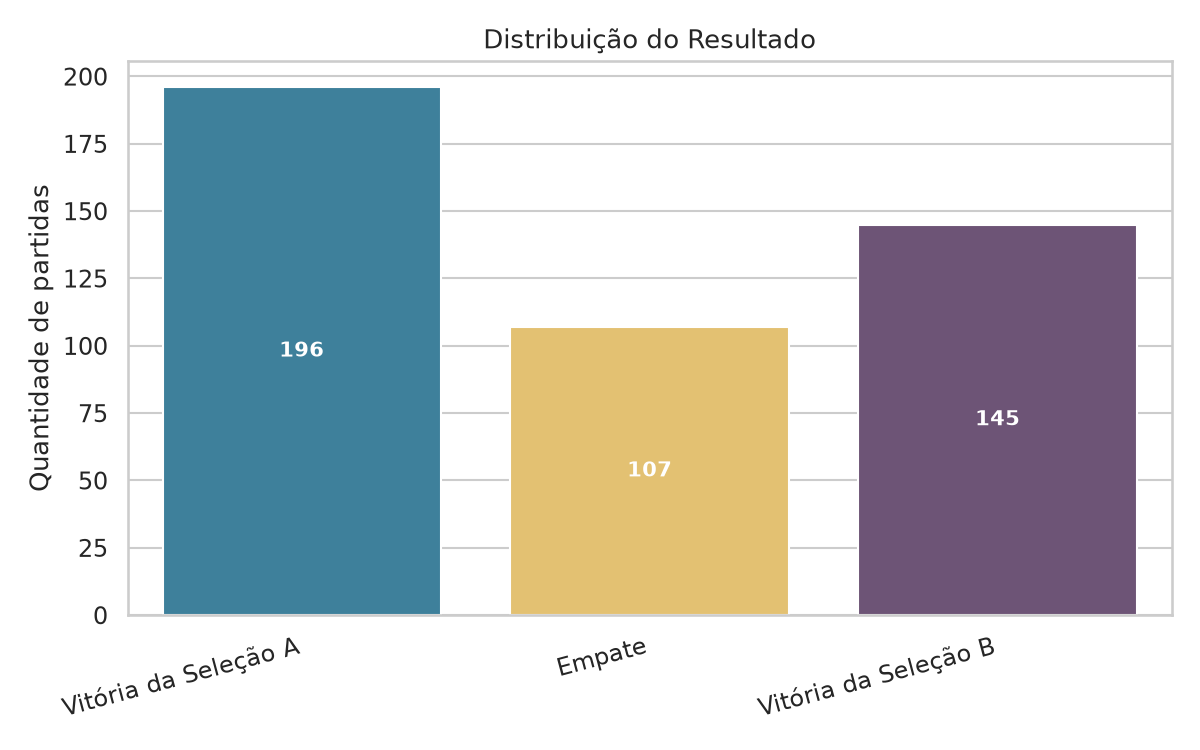
\includegraphics[width=0.75\textwidth]{analises/graficos/distribuicao_resultado.png}
    \caption{Distribuição geral das classes do alvo.}
    \label{fig:distribuicao_resultado}
\end{figure}

A classe mais frequente é vitória da Seleção A, com 196 partidas, seguida de
vitória da Seleção B, com 145 partidas, e empate, com 107 partidas. Isso mostra
que o problema não é perfeitamente balanceado, especialmente pela menor
frequência de empates.

O primeiro gráfico mostra que o empate é a classe menos frequente, representando
aproximadamente um quarto das partidas. Essa diferença é relevante porque um
modelo pode obter acurácia razoável prevendo mais vitórias do que empates, mas
ainda assim ter desempenho fraco na classe minoritária. Por isso, a análise
posterior considera macro-F1 como métrica central.

\begin{figure}[H]
    \centering
    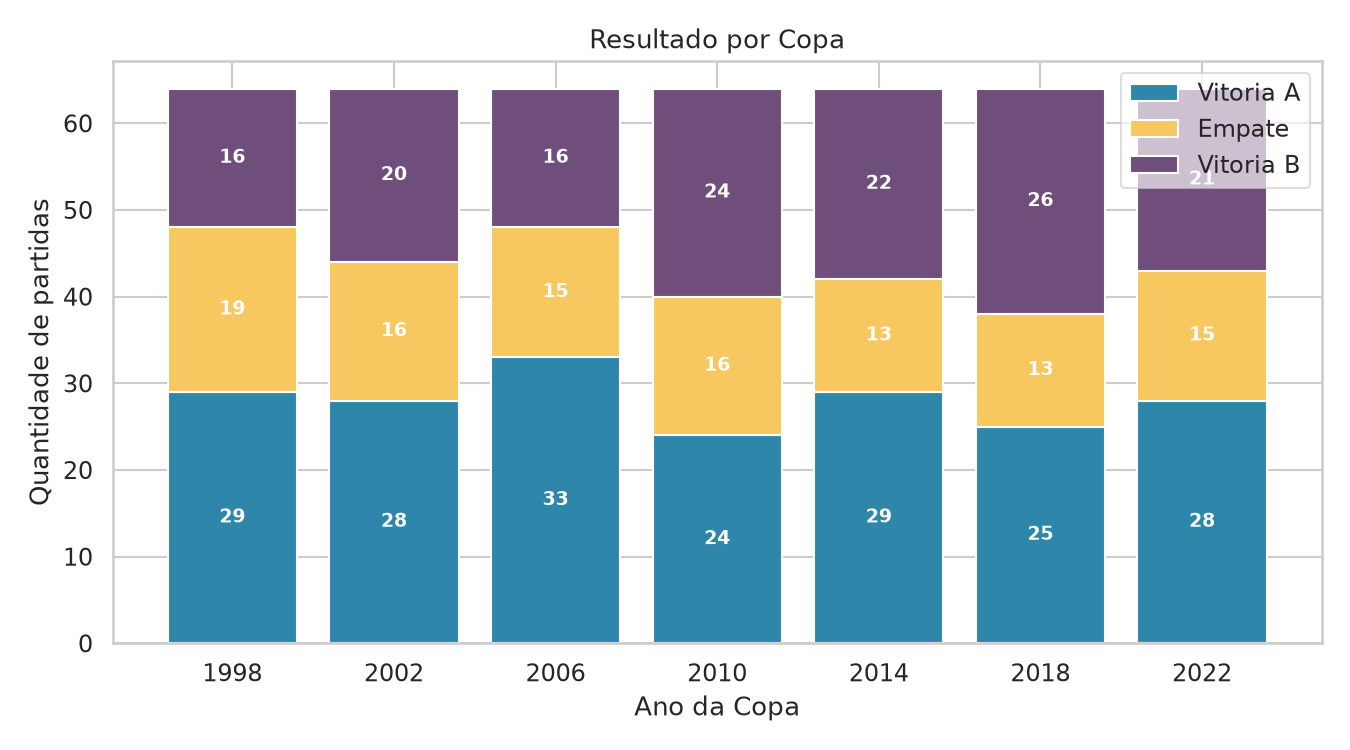
\includegraphics[width=0.85\textwidth]{analises/graficos/resultado_por_copa.png}
    \caption{Distribuição dos resultados por edição da Copa do Mundo.}
    \label{fig:resultado_por_copa}
\end{figure}

A Figura~\ref{fig:resultado_por_copa} mostra que a quantidade de empates varia
entre as edições, mas permanece menor que o total de vitórias. Essa característica
justifica o uso de macro-F1 como métrica principal.

O gráfico por Copa também indica que todas as edições têm o mesmo número de
partidas, o que facilita a comparação entre anos. Apesar disso, a distribuição
das classes muda de uma Copa para outra. Essa variação reforça a necessidade de
uma validação temporal, pois um modelo treinado em Copas anteriores precisa lidar
com mudanças naturais no padrão dos torneios seguintes.

\subsection{Ranking FIFA e Resultado}

Uma das relações mais relevantes observadas na análise exploratória foi entre a
diferença de ranking e o resultado da partida. Na Figura~\ref{fig:faixa_ranking},
valores negativos de diferença de ranking indicam vantagem para a Seleção A,
pois significam melhor posição no ranking FIFA.

As faixas foram definidas a partir de \texttt{diff\_rank}, calculado como
ranking da Seleção A menos ranking da Seleção B. Assim, ``A muito melhor''
representa diferença menor que -30 posições; ``A melhor'', entre -30 e -10;
``Equilibrado'', entre -10 e 10; ``B melhor'', entre 10 e 30; e ``B muito
melhor'', diferença maior que 30 posições.

\begin{figure}[H]
    \centering
    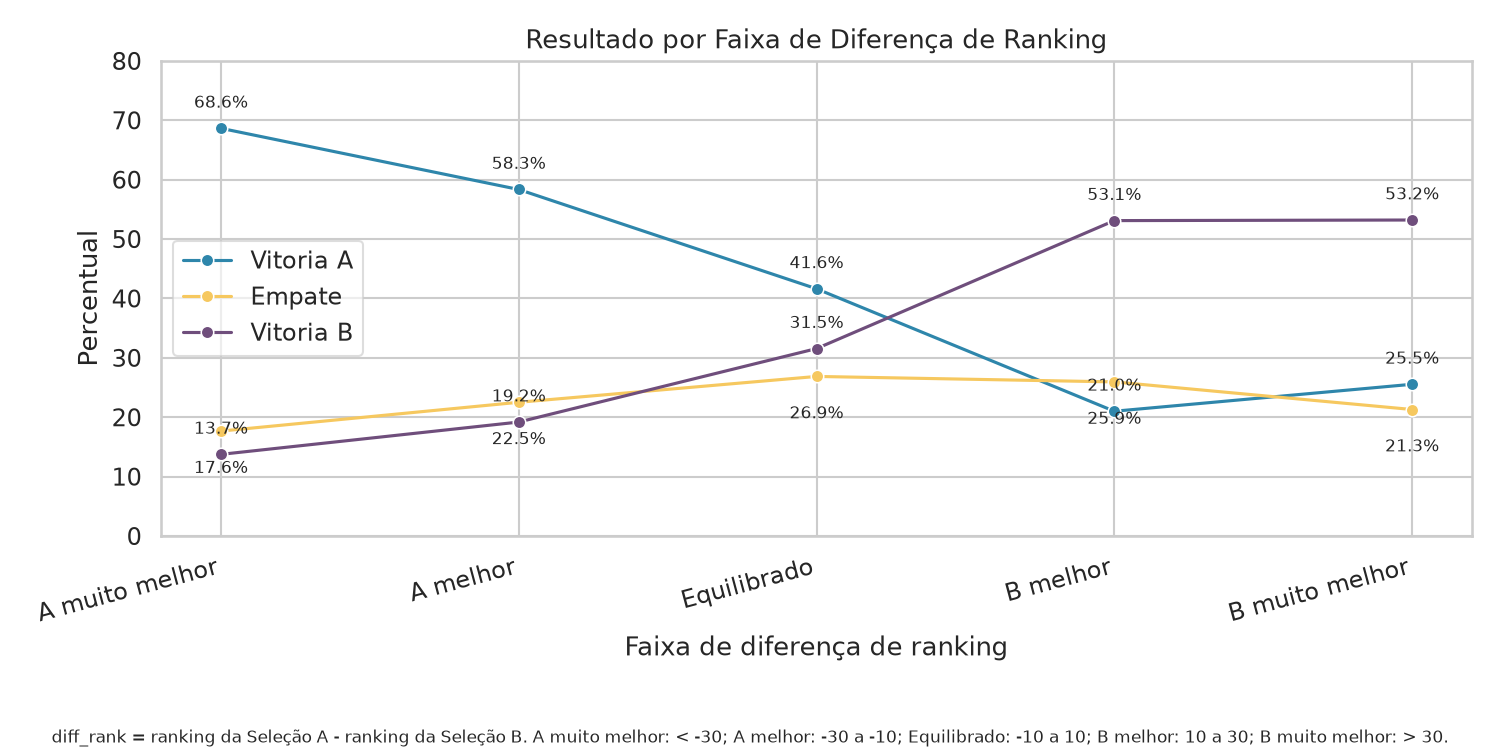
\includegraphics[width=0.9\textwidth]{analises/graficos/resultado_por_faixa_ranking.png}
    \caption{Resultado por faixa de diferença de ranking FIFA.}
    \label{fig:faixa_ranking}
\end{figure}

Quando a Seleção A estava muito melhor ranqueada, ela venceu 68,63\% das partidas
do grupo. Quando a Seleção B estava melhor ranqueada, a frequência de vitórias
da Seleção B aumentou. Esse resultado apoia a hipótese de que o ranking FIFA
possui relação relevante com o resultado das partidas.

Esse gráfico é o principal indício exploratório a favor da hipótese H1. A curva
de vitórias da Seleção A diminui conforme a vantagem de ranking passa para a
Seleção B, enquanto a curva de vitórias da Seleção B aumenta. O comportamento
não é perfeito, pois ainda existem empates e surpresas, mas a tendência geral é
coerente com a ideia de que a diferença de ranking contém informação preditiva.

\subsection{Resultados da Modelagem}

A Tabela~\ref{tab:modelos} apresenta os principais resultados dos modelos na
validação, no teste final e na avaliação adicional.

\begin{table}[H]
\centering
\caption{Desempenho dos modelos avaliados.}
\label{tab:modelos}
\begin{tabular}{llcc}
\toprule
Modelo & Conjunto & Acurácia & Macro-F1 \\
\midrule
Baseline & Validação 2014 & 0,4531 & 0,2079 \\
Baseline & Teste 2018 & 0,3906 & 0,1873 \\
Regressão logística & Validação 2014 & 0,4531 & 0,3789 \\
Regressão logística & Teste 2018 & 0,5000 & 0,4761 \\
Árvore de decisão & Validação 2014 & 0,3438 & 0,3524 \\
Árvore de decisão & Teste 2018 & 0,4062 & 0,3988 \\
Random forest & Validação 2014 & 0,4844 & 0,4127 \\
Random forest & Teste 2018 & 0,4219 & 0,3668 \\
\bottomrule
\end{tabular}
\end{table}

Na validação de 2014, o melhor modelo foi o random forest, com acurácia de
0,4844 e macro-F1 de 0,4127. No teste final de 2018, o melhor desempenho foi da
regressão logística, com acurácia de 0,5000 e macro-F1 de 0,4761.

\begin{figure}[H]
    \centering
    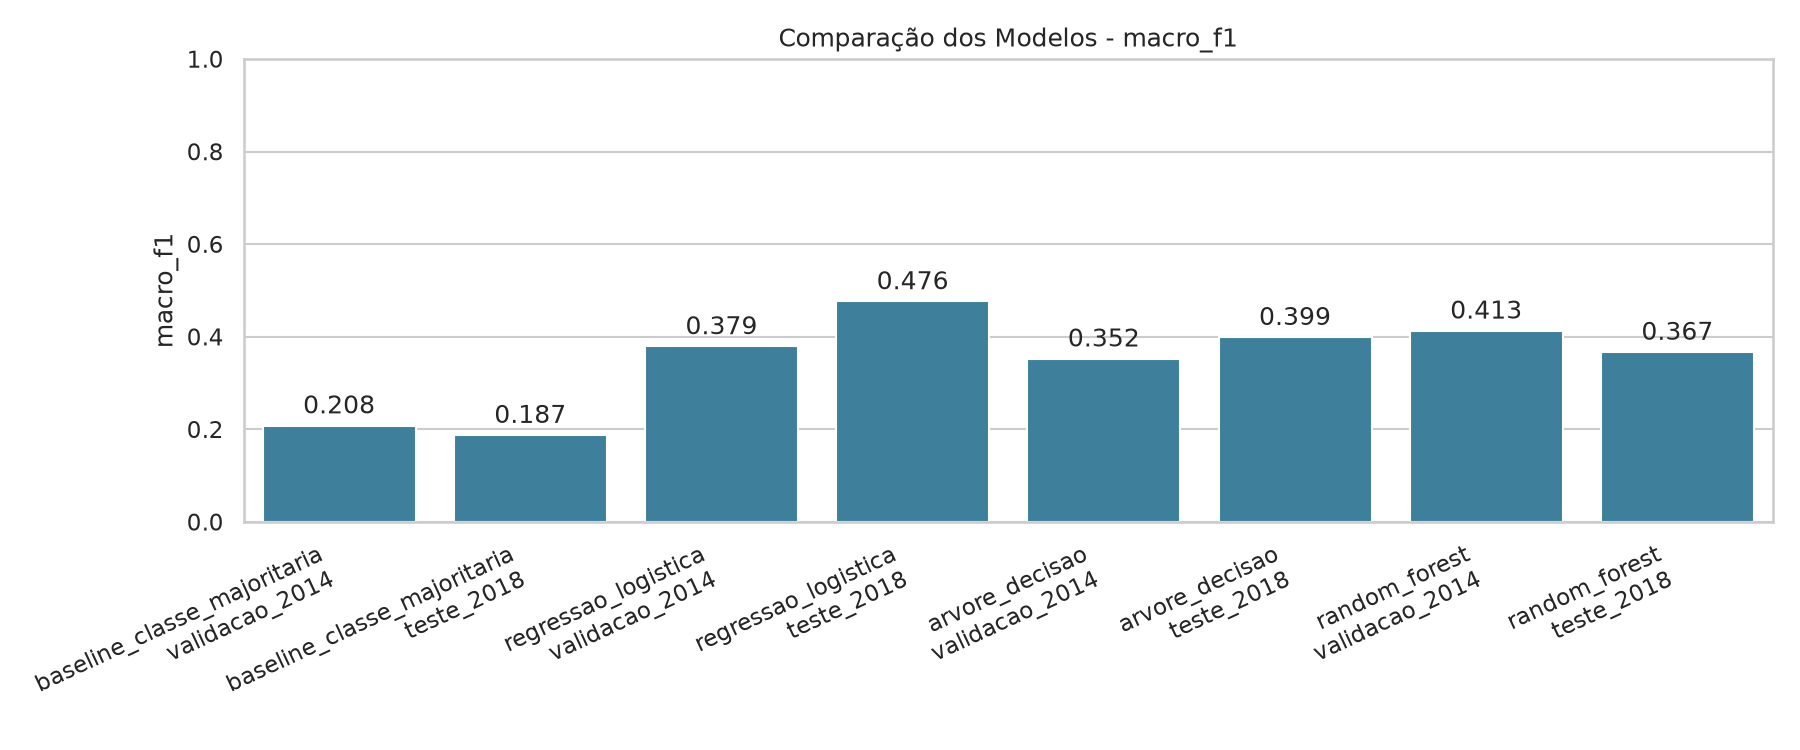
\includegraphics[width=0.95\textwidth]{modelagem/graficos/comparacao_modelos_macro_f1.png}
    \caption{Comparação dos modelos pela métrica macro-F1.}
    \label{fig:comparacao_macro_f1}
\end{figure}

Os modelos treinados superaram o baseline em macro-F1, indicando que os atributos
pré-Copa carregam algum sinal preditivo. Entretanto, os resultados também mostram
que a previsão de partidas de futebol continua sendo difícil.

\begin{figure}[H]
    \centering
    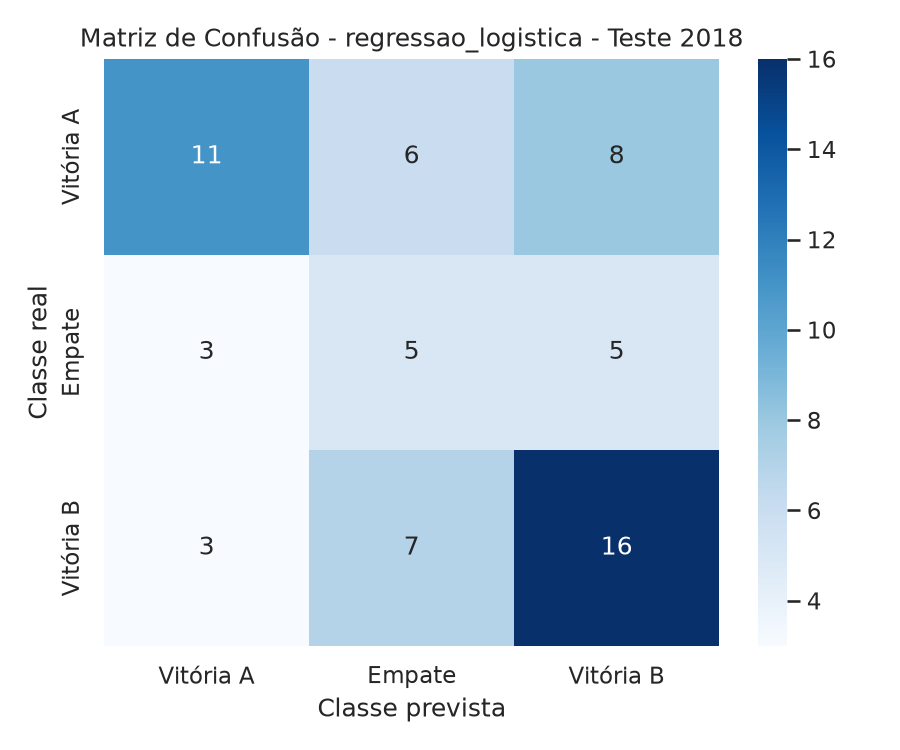
\includegraphics[width=0.7\textwidth]{modelagem/graficos/matriz_confusao_melhor_modelo_2018.png}
    \caption{Matriz de confusão do melhor modelo no teste de 2018.}
    \label{fig:matriz_confusao}
\end{figure}

A matriz de confusão indica que os erros se distribuem entre as três classes, com
maior dificuldade para prever empates. Esse comportamento é esperado, pois o
empate é uma classe menos frequente e mais sensível a eventos específicos da
partida.

\subsection{Avaliação das Hipóteses}

A Tabela~\ref{tab:hipoteses} apresenta a comparação dos grupos de atributos na
validação de 2014.

\begin{table}[H]
\centering
\caption{Avaliação dos grupos de atributos na validação de 2014.}
\label{tab:hipoteses}
\begin{tabular}{lccc}
\toprule
Grupo de atributos & Acurácia & Macro-F1 & Variáveis \\
\midrule
Ranking FIFA & 0,5938 & 0,4799 & 6 \\
Ranking + forma recente & 0,5312 & 0,4617 & 15 \\
Ranking + forma + ciclo & 0,4688 & 0,3931 & 28 \\
Completo sem força dos adversários & 0,4375 & 0,3887 & 29 \\
Modelo completo & 0,4531 & 0,3789 & 32 \\
\bottomrule
\end{tabular}
\end{table}

O melhor desempenho na validação ocorreu com o grupo de atributos de ranking
FIFA. Isso apoia a hipótese H1. A inclusão de forma recente e variáveis do ciclo
pré-Copa não melhorou o desempenho na validação, embora alguns grupos tenham
apresentado resultados competitivos no teste de 2018. Uma possível explicação é
o tamanho reduzido da amostra: o conjunto de treinamento possui apenas 256
partidas, o que torna modelos com muitos atributos mais sujeitos a ruído.

\begin{figure}[H]
    \centering
    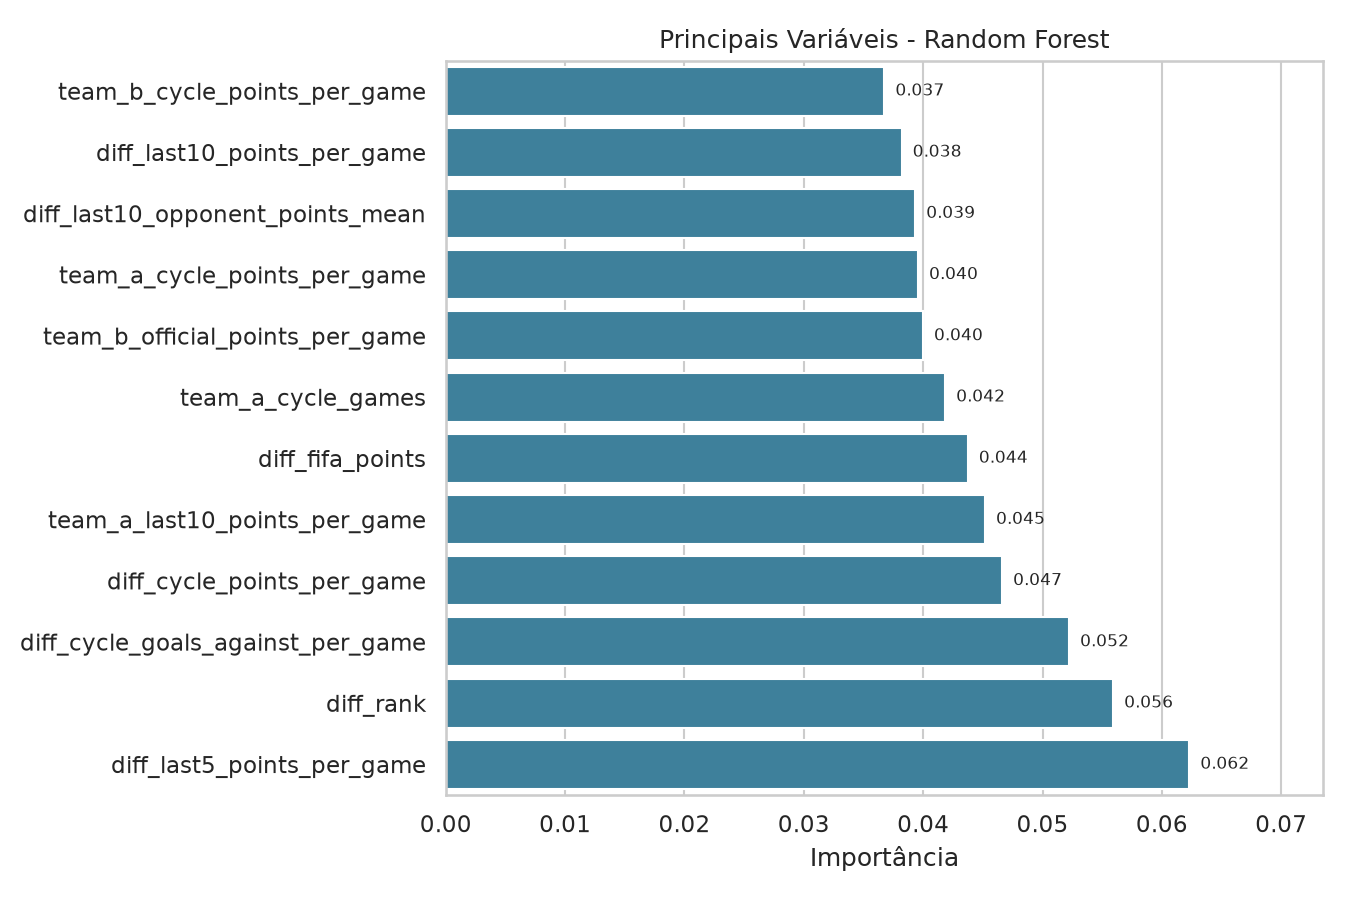
\includegraphics[width=0.85\textwidth]{modelagem/graficos/importancia_variaveis_random_forest.png}
    \caption{Principais variáveis segundo o random forest.}
    \label{fig:importancia_variaveis}
\end{figure}

A importância das variáveis reforça a presença de atributos ligados à força
relativa das seleções, como ranking, pontos FIFA e diferenças de desempenho.

Com base nos resultados, a H1 foi apoiada de forma mais clara, pois o grupo de
atributos de ranking apresentou o melhor desempenho na validação. A H2 recebeu
apoio parcial: a forma recente produziu desempenho próximo ao ranking isolado,
mas não superou a hipótese H1. A H3 também recebeu apoio parcial, pois alguns
resultados no teste de 2018 foram competitivos, mas a validação de 2014 não
indicou ganho consistente. A H4 não foi confirmada de forma clara, já que a
inclusão da força dos adversários não melhorou o modelo completo na validação.

\section{Discussão e Conclusão}

Os resultados indicam que é possível prever parcialmente resultados de partidas
da Copa do Mundo usando informações anteriores ao torneio. O desempenho dos
modelos treinados foi superior ao baseline, especialmente na métrica macro-F1.
No teste final de 2018, a regressão logística alcançou 50\% de acurácia e
macro-F1 de 0,4761.

A hipótese mais apoiada pelos dados foi a H1, relacionada ao ranking FIFA. O
grupo de atributos de ranking obteve o melhor resultado na validação de 2014,
com acurácia de 0,5938 e macro-F1 de 0,4799. Isso sugere que a força geral das
seleções, medida pelo ranking, é um dos fatores mais úteis para a predição.

Por outro lado, a inclusão de muitas variáveis de forma recente e ciclo pré-Copa
não garantiu melhora consistente. Esse resultado não significa que essas
variáveis sejam irrelevantes no futebol, mas indica que, neste dataset, sua
utilidade preditiva foi limitada. Uma explicação provável é o tamanho reduzido da
amostra, já que Copas do Mundo possuem poucas partidas quando comparadas a outros
contextos de aprendizado de máquina.

As principais limitações do trabalho são:

\begin{itemize}
    \item número reduzido de partidas disponíveis;
    \item ausência de variáveis contextuais, como escalações, lesões e local
    específico da partida;
    \item dificuldade natural de prever empates;
    \item possível variação do significado do ranking FIFA ao longo dos anos.
\end{itemize}

Como melhorias futuras, poderiam ser incluídos dados de jogadores, estatísticas
avançadas das partidas, probabilidades de mercado e modelos probabilísticos.
Também seria possível reformular o problema para prever apenas vitória ou não
vitória, ou simular cenários específicos, como apostas em que o empate anula a
previsão.

Conclui-se que o dataset derivado e os modelos avaliados fornecem uma base
adequada para investigar fatores associados ao desempenho na Copa do Mundo. O
ranking FIFA se mostrou o fator mais consistente, enquanto os demais atributos
pré-Copa exigem cautela devido ao risco de sobreajuste e à alta variabilidade do
futebol.

\section*{Referências e Bases de Dados}

\begin{itemize}
    \item Mart Jürisoo. \textit{International football results from 1872 to
    2026}. Kaggle. Disponível em:
    \url{https://www.kaggle.com/datasets/martj42/international-football-results-from-1872-to-2017}.
    \item Lucas Yukio Imafuko. \textit{FIFA Men's World Ranking}. Kaggle.
    Disponível em:
    \url{https://www.kaggle.com/datasets/lucasyukioimafuko/fifa-mens-world-ranking}.
    \item Scikit-learn. \textit{User Guide: supervised learning and model
    evaluation}. Disponível em: \url{https://scikit-learn.org/stable/user_guide.html}.
    \item Hastie, T.; Tibshirani, R.; Friedman, J. \textit{The Elements of
    Statistical Learning}. Springer.
    \item James, G.; Witten, D.; Hastie, T.; Tibshirani, R. \textit{An
    Introduction to Statistical Learning}. Springer.
\end{itemize}

\end{document}
